\documentclass[11pt]{article}
\usepackage[utf8]{inputenc}
\usepackage[margin=1in]{geometry}
\usepackage{graphicx}
\usepackage{amsmath}
\usepackage{booktabs}
\usepackage{tikz}
\usetikzlibrary{arrows.meta, positioning, fit, backgrounds}
\usepackage{hyperref}
\usepackage{caption}
\usepackage{float}
\usepackage{xcolor}
\usepackage{tablefootnote}

\title{Evaluating DPO's Implicit Reward as a Preference Scorer\\
Under Distribution Shift}
\author{%
\begin{tabular}{c@{\hspace{7mm}}c@{\hspace{7mm}}c}
Shamima Hossain & Laila Sumiya Khan Nilo & Abdullah Al Mahmud \\
ID 21141119 & ID 17301022 & ID 17301033
\end{tabular}}
\date{}

\begin{document}

\maketitle

\begin{abstract}
Direct Preference Optimization (DPO) claims to skip the reward-model stage of RLHF entirely: a
DPO-trained policy is itself, implicitly, a reward model. We test this claim as a
preference-ranking task. Under a training budget matched between conditions, we train a
Qwen2.5-0.5B policy with LoRA from one shared SFT checkpoint into three scorers --- a DPO
policy's implicit reward, an explicitly trained Bradley--Terry reward model, and an SFT
log-probability baseline with no reward-specific training --- and evaluate all three as
pairwise classifiers in distribution, on four RewardBench distribution-shift subsets, and on a
cross-dataset shift set, across five seeds. In distribution, the explicit reward model wins
(0.663 vs.\ 0.600 length-controlled accuracy, all five seed-level McNemar tests significant):
\textbf{H1 is supported}. Out of distribution the predicted widening does not occur; where a
resolvable difference exists (two of five shifted sets), it favors the implicit reward instead:
\textbf{H2 is not supported}. On the hardest subsets, the SFT baseline beats both trained
scorers. An extended four-epoch run and a per-checkpoint bias-drift analysis confirm the
in-distribution ranking is not an artifact of stopping early, and implicate a length-preference
confound in part of that gap.
\end{abstract}

\section{Introduction}

Reinforcement Learning from Human Feedback (RLHF) is the standard recipe for aligning a
pretrained language model with human preferences: collect pairwise comparisons between
candidate responses, train an explicit reward model to predict which response people
preferred, and then optimize the policy against that learned reward with reinforcement learning
(typically PPO), subject to a KL penalty that keeps the policy close to a reference
model~\cite{christiano2017deep, ouyang2022instructgpt}. That pipeline needs a separately
trained reward model and an unstable, hyperparameter-sensitive reinforcement-learning stage.
Direct Preference Optimization (DPO)~\cite{rafailov2023dpo} was proposed to skip both, training
a policy directly on preference pairs with a simple supervised-style loss while implicitly
optimizing the same KL-regularized objective; its title makes the strong version of the claim,
that a DPO-trained policy \emph{is}, secretly, also a reward model. That reward is recoverable
as $\hat r(x,y) = \beta\log[\pi_\theta(y\mid x)/\pi_{\mathrm{ref}}(y\mid x)]$, but the
equivalence is exact only at the optimum, which a trained policy is not guaranteed to reach;
what we test here is $\hat r$ as a practical preference scorer, in and out of distribution, not
the theorem itself.

Christiano et al.~\cite{christiano2017deep} introduced the core idea of learning a reward
function from pairwise human preferences and optimizing a policy against it with reinforcement
learning; its strength is generality (only comparative, not absolute, feedback is needed), but
routing through PPO makes the resulting pipeline sensitive to reward-model quality and prone to
reward hacking under prolonged optimization. Ouyang et al.~\cite{ouyang2022instructgpt} scaled
this to language models with InstructGPT, explicitly training a Bradley--Terry-style reward
model~\cite{bradley1952rank} and then fine-tuning the policy against it; the alignment gains
were large, but the paper documents the same PPO instability and adds the cost of training and
serving a separate reward model. Gao et al.~\cite{gao2023overoptimization} quantify how far a
learned reward can be optimized before proxy and true reward diverge --- the failure our
held-out comparison probes --- though their scaling laws are fitted against synthetic gold
reward models rather than human labels. DPO~\cite{rafailov2023dpo} removes that stage by training the
policy directly on preference pairs with a simpler, more stable loss; its limitation, as
detailed above, is that it discards the reward model as an explicit, separately-evaluable
object, so any downstream reuse of $\hat r$ as a scorer has not been validated the way an
explicit reward model would be, and we did not identify prior work that directly compares its
preference-ranking performance against an explicitly trained reward model under matched
training conditions. SimPO~\cite{meng2024simpo} is one of several post-DPO variants that drop
the reference policy for a length-normalized reward, saving memory and curbing length bias, but
in doing so it removes the very $\pi_\theta/\pi_{\mathrm{ref}}$ ratio whose reuse as a reward
model we test here. RewardBench~\cite{lambert2024rewardbench} is the closest prior work to a
stress test of reward models, built around adversarial, distribution-shifted comparisons, but
it evaluates only explicitly-trained reward models, not policies read out as implicit ones.
Two further ingredients make our question tractable at small scale: LoRA~\cite{hu2022lora}
allows several full training conditions to be run and compared on a single consumer GPU, at the
cost of not testing full-parameter fine-tuning; and UltraFeedback~\cite{cui2023ultrafeedback}
supplies the large, AI-scored preference pool our budget-matched training draws from, though its
preferences reflect an AI judge's biases rather than human raters' directly.

This gap matters practically: if the implicit reward generalizes as well as an explicit one,
DPO checkpoints could be reused as reward models, removing a training stage from the RLHF
pipeline; if it does not, the ``secretly a reward model'' framing needs the qualification that
it holds only in a narrow, training-distribution sense. We test two pre-registered hypotheses:
\textbf{H1}, the explicit reward model beats the implicit reward on held-out in-distribution
pairs, and \textbf{H2}, that gap widens under distribution shift. We treat a null result
(implicit $\approx$ explicit) as equally publishable, since it would itself substantiate DPO's
claim empirically at small scale.

\subsection{Our Contribution}
\begin{itemize}
  \item \textbf{Budget-matched pipeline:} the DPO policy and the explicit reward model differ
    only in their loss (Figure~\ref{fig:pipeline}).
  \item \textbf{Correctness pass:} four silent bugs found and fixed, and the implicit-reward
    extraction verified against the DPO trainer's own computation (\S\ref{sec:pipeline-check}).
  \item \textbf{Evaluation:} both scorers, plus an SFT log-probability baseline, scored as
    pairwise classifiers across six test sets over five seeds (\S\ref{sec:eval}).
  \item \textbf{Ablations:} a four-epoch extended-training run and a per-checkpoint
    length-bias-drift analysis (\S\ref{sec:ablations}).
\end{itemize}

\section{Material and Methods}

\subsection{Overview}
Figure~\ref{fig:pipeline} shows the overall pipeline. A single supervised fine-tuning (SFT)
pass produces the shared reference policy $\pi_{\mathrm{ref}}$. Two training conditions then
branch off from that identical starting point: DPO produces a policy $\pi_\theta$ from which the
implicit reward is read off after training with no further reward-specific training, and a
Bradley--Terry reward model is trained explicitly on the same pairs. Both are evaluated as
pairwise preference classifiers on held-out data.

\begin{figure}[H]
\centering
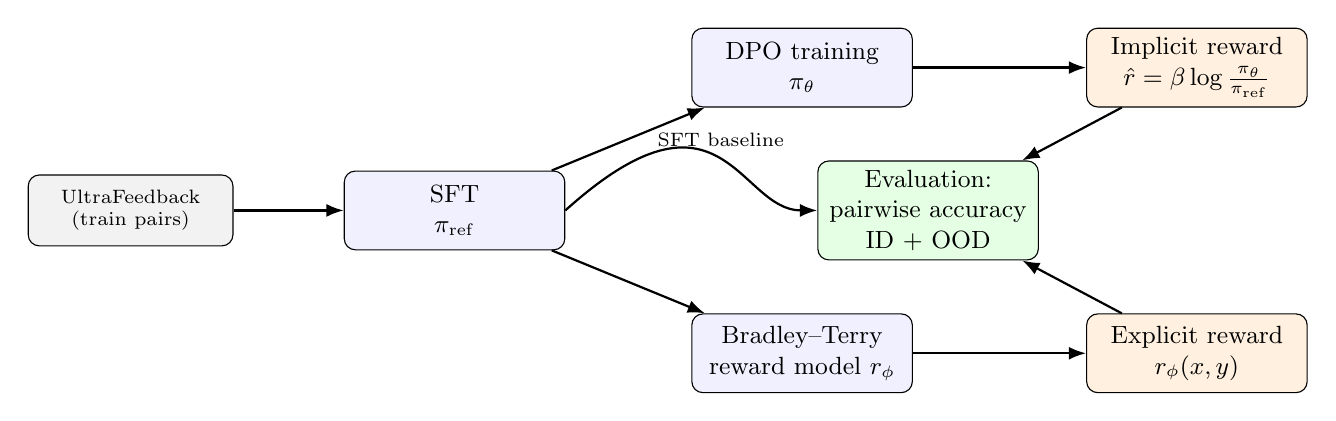
\begin{tikzpicture}[
  node distance=10mm and 14mm,
  box/.style={draw, rounded corners, align=center, minimum height=10mm, minimum width=28mm,
              font=\small, fill=blue!6},
  data/.style={draw, rounded corners, align=center, minimum height=9mm, minimum width=26mm,
               font=\scriptsize, fill=gray!10},
  arr/.style={-{Latex[length=2.2mm]}, thick}
]
  \node[data] (data) {UltraFeedback\\(train pairs)};
  \node[box, right=of data] (sft) {SFT\\$\pi_{\mathrm{ref}}$};
  \node[box, above right=8mm and 16mm of sft] (dpo) {DPO training\\$\pi_\theta$};
  \node[box, below right=8mm and 16mm of sft] (rm) {Bradley--Terry\\reward model $r_\phi$};
  \node[box, right=22mm of dpo, fill=orange!12] (implicit) {Implicit reward\\$\hat r=\beta\log\frac{\pi_\theta}{\pi_{\mathrm{ref}}}$};
  \node[box, right=22mm of rm, fill=orange!12] (explicit) {Explicit reward\\$r_\phi(x,y)$};
  \node[box, right=32mm of sft, fill=green!10, yshift=0mm] (eval) {Evaluation:\\pairwise accuracy\\ID + OOD};

  \draw[arr] (data) -- (sft);
  \draw[arr] (sft) -- (dpo);
  \draw[arr] (sft) -- (rm);
  \draw[arr] (dpo) -- (implicit);
  \draw[arr] (rm) -- (explicit);
  \draw[arr] (implicit) -- (eval);
  \draw[arr] (explicit) -- (eval);
  \draw[arr] (sft.east) .. controls +(20mm,18mm) and +(-10mm,0mm) .. (eval.west)
    node[midway, above, font=\scriptsize] {SFT baseline};
\end{tikzpicture}
\caption{Pipeline overview. \emph{Budget-matched} means both conditions share one SFT
checkpoint, the same preference pairs, LoRA configuration, effective batch size, and optimizer
steps; only the loss differs. $\pi_{\mathrm{ref}}$ is also scored directly, as the SFT
log-probability baseline.}
\label{fig:pipeline}
\end{figure}

\subsection{Dataset Description}
\label{sec:dataset}
All data are established public benchmarks (Table~\ref{tab:datasets}). UltraFeedback~\cite{
cui2023ultrafeedback} supplies both the training pairs and the in-distribution held-out test
set. RewardBench~\cite{lambert2024rewardbench} supplies four distribution-shift subsets ---
Chat, Chat-Hard, Safety, and Reasoning --- built specifically to stress-test reward models on
harder and adversarially-constructed comparisons. Anthropic's HH-RLHF (harmless-base split)
supplies a cross-dataset shift test, since it comes from a different data-collection process
entirely. Every example is normalized to the same (\emph{prompt}, \emph{chosen},
\emph{rejected}) schema. Training pairs for the matched comparison are drawn from a common
length-eligible pool so both conditions see the identical first 8,000 examples
(Table~\ref{tab:bugs} details why this pool is necessary).

\begin{table}[H]
\centering
\caption{Evaluation sets. ``Length-matched'' counts the pairs surviving the 1.2 length-ratio
filter (\S\ref{sec:eval}); the three marked $^\dagger$ fall below 100 (\S\ref{sec:threats}).}
\label{tab:datasets}
\begin{tabular}{lllrr}
\toprule
Set & Role & Distribution & Pairs & Length-matched \\
\midrule
UltraFeedback & training + ID test & in-distribution & 1{,}997 & 442 \\
RewardBench: Chat & OOD test & distribution shift & 358 & 32$^\dagger$ \\
RewardBench: Chat-Hard & OOD test & distribution shift & 456 & 62$^\dagger$ \\
RewardBench: Safety & OOD test & distribution shift & 740 & 83$^\dagger$ \\
RewardBench: Reasoning & OOD test & distribution shift & 1{,}431 & 908 \\
HH-RLHF (harmless) & OOD test & cross-dataset shift & 2{,}312 & 276 \\
\bottomrule
\end{tabular}
\end{table}

\subsection{Tools, Models, and Algorithms Used}
\label{sec:tools}
The base model for every condition is Qwen2.5-0.5B, a small, publicly available
instruction-capable language model, chosen so that all three training conditions plus the
extended-training ablation fit on a single 24\,GB GPU (NVIDIA A10G). All fine-tuning uses
Low-Rank Adaptation (LoRA)~\cite{hu2022lora} with rank $r=16$, $\alpha=32$, dropout $0.05$,
applied to every attention and MLP projection matrix, via HuggingFace's TRL library. The shared
reference policy $\pi_{\mathrm{ref}}$ is produced by one epoch of SFT on the \emph{chosen}
responses from 32,000 length-eligible UltraFeedback pairs (1,998 optimizer steps). ($\pi_{
\mathrm{ref}}$ is a shared input to the matched comparison, not one of the compared conditions,
so it is not budget-limited.) Figure~\ref{fig:models} summarizes the three training objectives.

\begin{figure}[H]
\centering
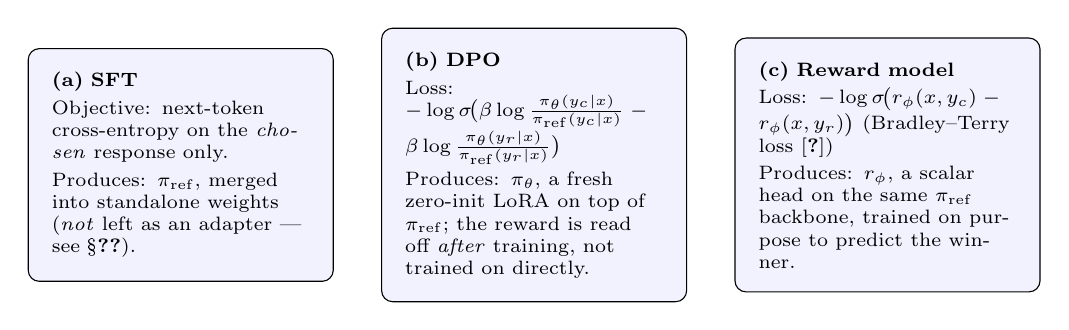
\begin{tikzpicture}[
  box/.style={draw, rounded corners, align=left, minimum width=0.29\linewidth,
              font=\scriptsize, fill=blue!5, text width=0.27\linewidth, inner sep=3mm},
  lbl/.style={font=\bfseries\small}
]
  \node[box] (a) at (0,0) {
    \textbf{(a) SFT} \\[2pt]
    Objective: next-token cross-entropy on the \emph{chosen} response only. \\[2pt]
    Produces: $\pi_{\mathrm{ref}}$, merged into standalone weights (\emph{not} left as an
    adapter --- see \S\ref{sec:pipeline-check}).
  };
  \node[box, right=6mm of a] (b) {
    \textbf{(b) DPO} \\[2pt]
    Loss: $-\log\sigma\!\big(\beta\log\tfrac{\pi_\theta(y_c|x)}{\pi_{\mathrm{ref}}(y_c|x)}
    -\beta\log\tfrac{\pi_\theta(y_r|x)}{\pi_{\mathrm{ref}}(y_r|x)}\big)$ \\[2pt]
    Produces: $\pi_\theta$, a fresh zero-init LoRA on top of $\pi_{\mathrm{ref}}$; the reward is
    read off \emph{after} training, not trained on directly.
  };
  \node[box, right=6mm of b] (c) {
    \textbf{(c) Reward model} \\[2pt]
    Loss: $-\log\sigma\!\big(r_\phi(x,y_c)-r_\phi(x,y_r)\big)$ (Bradley--Terry
    loss \cite{bradley1952rank}) \\[2pt]
    Produces: $r_\phi$, a scalar head on the same $\pi_{\mathrm{ref}}$ backbone, trained on
    purpose to predict the winner.
  };
\end{tikzpicture}
\caption{The three training objectives, all starting from the identical $\pi_{\mathrm{ref}}$
checkpoint produced by (a).}
\label{fig:models}
\end{figure}

Table~\ref{tab:hparams} lists the hyperparameters shared across SFT, DPO, and the reward model;
the only quantities that differ between the two conditions are the loss function itself and,
for the extended-training ablation, the number of epochs.

\begin{table}[H]
\centering
\caption{Shared hyperparameters; $\beta=0.1$ is DPO's implicit-reward temperature.}
\label{tab:hparams}
\begin{tabular}{ll}
\toprule
Base model & Qwen2.5-0.5B \\
LoRA rank / $\alpha$ / dropout & 16 / 32 / 0.05 \\
LoRA target modules & q,k,v,o,gate,up,down projections \\
Effective batch size & 16 (batch 4 $\times$ grad.\ accum.\ 4) \\
Learning rate (SFT / DPO \& RM) & $2\times10^{-4}$ / $5\times10^{-5}$, cosine schedule \\
Precision & bf16 (single NVIDIA A10G) \\
Training pairs (headline run) & 8{,}000, budget-matched, 1 epoch \\
DPO $\beta$ (headline run) & 0.1 \\
Seeds (headline run) & 5 \\
Extended-training ablation & 4 epochs, 2 seeds, held-out eval every 100 steps \\
\bottomrule
\end{tabular}
\end{table}

\subsection{Performance Evaluation}
\label{sec:eval}
Every trained scorer produces a scalar $s(x,y)$: for the implicit reward, $s = \hat r =
\beta\log[\pi_\theta(y\mid x)/\pi_{\mathrm{ref}}(y\mid x)]$; for the reward model, $s =
r_\phi(x,y)$; for the SFT baseline, $s = \log\pi_{\mathrm{ref}}(y\mid x)$. Each $s$ is used only
for ranking --- the scorer's decision is the sign of $s(x,y_c)-s(x,y_r)$ --- and \emph{pairwise
accuracy}, the fraction of pairs ranked correctly, is the primary outcome.

\emph{Length-controlled accuracy} restricts this to pairs with $\max(L_c,L_r)/\max(1,
\min(L_c,L_r)) \le 1.2$, where $L_c,L_r$ are character lengths of the response text (prompt
excluded, un-tokenized); this filter is aggressive on the smaller RewardBench subsets. We also
report non-neural floors (random, pick-longer, TF-IDF+LR) with no language-model fine-tuning,
for comparison alongside the SFT baseline.

\emph{ECE} is computed over 10 equal-width confidence bins, per seed on the full test set (not
length-controlled) and averaged. \emph{McNemar's exact test} (a binomial test on the discordant pairs) is run separately per
seed between the implicit and explicit scorers; we report the resulting range of five p-values
rather than their mean, since independent p-values should not be averaged. The reported 95\%
CI is $\bar x \pm t_{0.975,4}\,s/\sqrt5$ over the five seed-level values of a given (test set,
scorer, metric) triple, where $s$ is their sample standard deviation (\S\ref{sec:threats}
discusses what this interval does and does not capture). We write \emph{CI excludes/includes 0}
for whether a paired explicit-minus-implicit difference is resolvable at this sample size.

\section{Experimental Analysis}

\noindent Code, configuration files, and the full pipeline used to produce every number and
figure below are available at \url{https://github.com/silvererudite/dpo-implicit-reward}, with
every per-pair score persisted to disk so every number below is recomputable without re-running
any model.

\subsection{Non-neural reference floors}
Table~\ref{tab:baselines} shows the zero-training reference floors. Pick-longer wins
RewardBench-Chat (0.805) but collapses on Chat-Hard (0.294), which inverts that cue by
construction, so raw accuracy on these benchmarks is substantially a length signal; this
motivates length-controlled accuracy as the primary metric below. TF-IDF+LR lands
below chance on Reasoning (0.282), suggesting the lexical cues it relies on are actively
misleading on that subset.

\begin{table}[H]
\centering
\caption{Non-neural reference floors (pairwise accuracy, no language-model training; TF-IDF+LR
does fit a logistic regression). Pick-shorter is omitted as it is exactly $1-$pick-longer.}
\label{tab:baselines}
\begin{tabular}{lrrr}
\toprule
Test set & Random & Pick-longer & TF-IDF + LR \\
\midrule
UltraFeedback (ID) & 0.500 & 0.568 & 0.618 \\
RewardBench: Chat & 0.500 & 0.805 & 0.754 \\
RewardBench: Chat-Hard & 0.500 & 0.294 & 0.382 \\
RewardBench: Safety & 0.500 & 0.420 & 0.450 \\
RewardBench: Reasoning & 0.500 & 0.397 & 0.282 \\
HH-RLHF (harmless) & 0.500 & 0.445 & 0.453 \\
\bottomrule
\end{tabular}
\end{table}

\subsection{Pipeline correctness pass}
\label{sec:pipeline-check}
We cross-checked our implicit-reward extraction against TRL's own internal DPO reward
computation on a batch of trained-on pairs, on five points:
(i) our tokenization matches TRL's token-for-token;
(ii) our per-pair values agree with TRL's logged ones up to a small residual attributable to
batching and floating point (padded batched forward passes inside TRL versus our unpadded
per-example ones);
(iii) the extracted reward is exactly linear in $\beta$, ruling out a scaling bug;
(iv) an unmasked-prompt control shifts the reward far more than that residual, ruling out a
masking bug by comparison;
(v) $\pi_{\mathrm{ref}}$ is bit-identical to TRL's adapter-disabled reference.
The residual's exact source is not characterized, but it does not affect the reported metrics:
pairwise accuracy depends only on the \emph{sign} of each scorer's own difference.

Bringing up the training pipeline separately surfaced four correctness bugs, none of which
crashed --- all would have produced plausible, wrong results (Table~\ref{tab:bugs}).

\begin{table}[H]
\centering
\small
\caption{Correctness bugs found and fixed before trusting any result. The first two fixes are
why the SFT adapter is merged into standalone weights rather than left live beneath
DPO/reward-model training.}
\label{tab:bugs}
\begin{tabular}{p{2.6cm}p{4.3cm}p{4.3cm}p{2.8cm}}
\toprule
Bug & Symptom if unfixed & Fix & Verified by \\
\midrule
Wrong $\pi_{\mathrm{ref}}$ & DPO trains against the raw base model, not the SFT policy &
  Merge the SFT adapter into the base weights before DPO/RM & DPO loss starts at exactly $\ln 2$ \\
Frozen RM head & Scalar head stays at random init; training does nothing to it &
  Merge SFT first, then attach a fresh sequence-classification head & \texttt{trainable == True} (measured) \\
Train-pair mismatch & RewardTrainer drops long pairs, DPOTrainer truncates them --- 7{,}520 vs.\ 8{,}000 pairs at the same nominal budget &
  Draw both trainers from one common length-eligible pool & Pool hash-identical between runs \\
Multi-GPU batch inflation & HF \texttt{Trainer} auto-wraps in \texttt{DataParallel}; effective batch silently $4\times$ larger &
  Pin every run to a single GPU & --- \\
\bottomrule
\end{tabular}
\end{table}

\subsection{H1: in-distribution comparison}
In distribution, the explicit reward model wins (Table~\ref{tab:results}) in every individual
seed, with all five seed-level McNemar tests significant ($p<0.0001$--$0.0019$).
\textbf{H1 is supported.}

\begin{table}[H]
\centering
\caption{Length-controlled pairwise accuracy (mean $\pm$ 95\% CI, 5 seeds). ``Diff.'' is
explicit minus implicit, paired within each seed.\tablefootnote{Computed from unrounded
per-seed values, so it can differ by up to 0.001 from the rounded means shown.} ``95\% CI
excludes/includes 0'' is defined in \S\ref{sec:eval}; a negative, CI-excludes-0 difference means
the implicit reward is ahead.}
\label{tab:results}
\small
\begin{tabular}{lrrrrl}
\toprule
Test set & DPO implicit & Explicit RM & SFT baseline & Diff.\ (E$-$I) & 95\% CI \\
\midrule
UltraFeedback (ID)      & 0.600 $\pm$ 0.026 & 0.663 $\pm$ 0.009 & 0.529 & $+0.062\pm0.030$ & excl.\ 0 \\
RewardBench: Chat        & 0.800 $\pm$ 0.044 & 0.747 $\pm$ 0.080 & 0.500 & $-0.053\pm0.058$ & incl.\ 0 \\
RewardBench: Chat-Hard   & 0.535 $\pm$ 0.052 & 0.615 $\pm$ 0.061 & 0.661 & $+0.079\pm0.109$ & incl.\ 0 \\
RewardBench: Safety      & 0.492 $\pm$ 0.036 & 0.549 $\pm$ 0.059 & 0.530 & $+0.058\pm0.074$ & incl.\ 0 \\
RewardBench: Reasoning   & 0.850 $\pm$ 0.003 & 0.663 $\pm$ 0.019 & 0.906 & $-0.187\pm0.020$ & excl.\ 0 \\
HH-RLHF (harmless)       & 0.472 $\pm$ 0.016 & 0.429 $\pm$ 0.036 & 0.435 & $-0.043\pm0.030$ & excl.\ 0 \\
\bottomrule
\end{tabular}
\end{table}

\subsection{H2: does the gap widen out of distribution?}
Pairing the explicit-minus-implicit difference \emph{within} each seed, so run-to-run variance
cancels, three of five OOD sets show no resolvable difference (Chat, Chat-Hard, Safety); on the
two that do, Reasoning and HH-RLHF, the difference runs opposite to H2, favoring the implicit
reward (Figure~\ref{fig:paired-delta}, Table~\ref{tab:results}). \textbf{H2 is not supported.}

\begin{figure}[H]
\centering
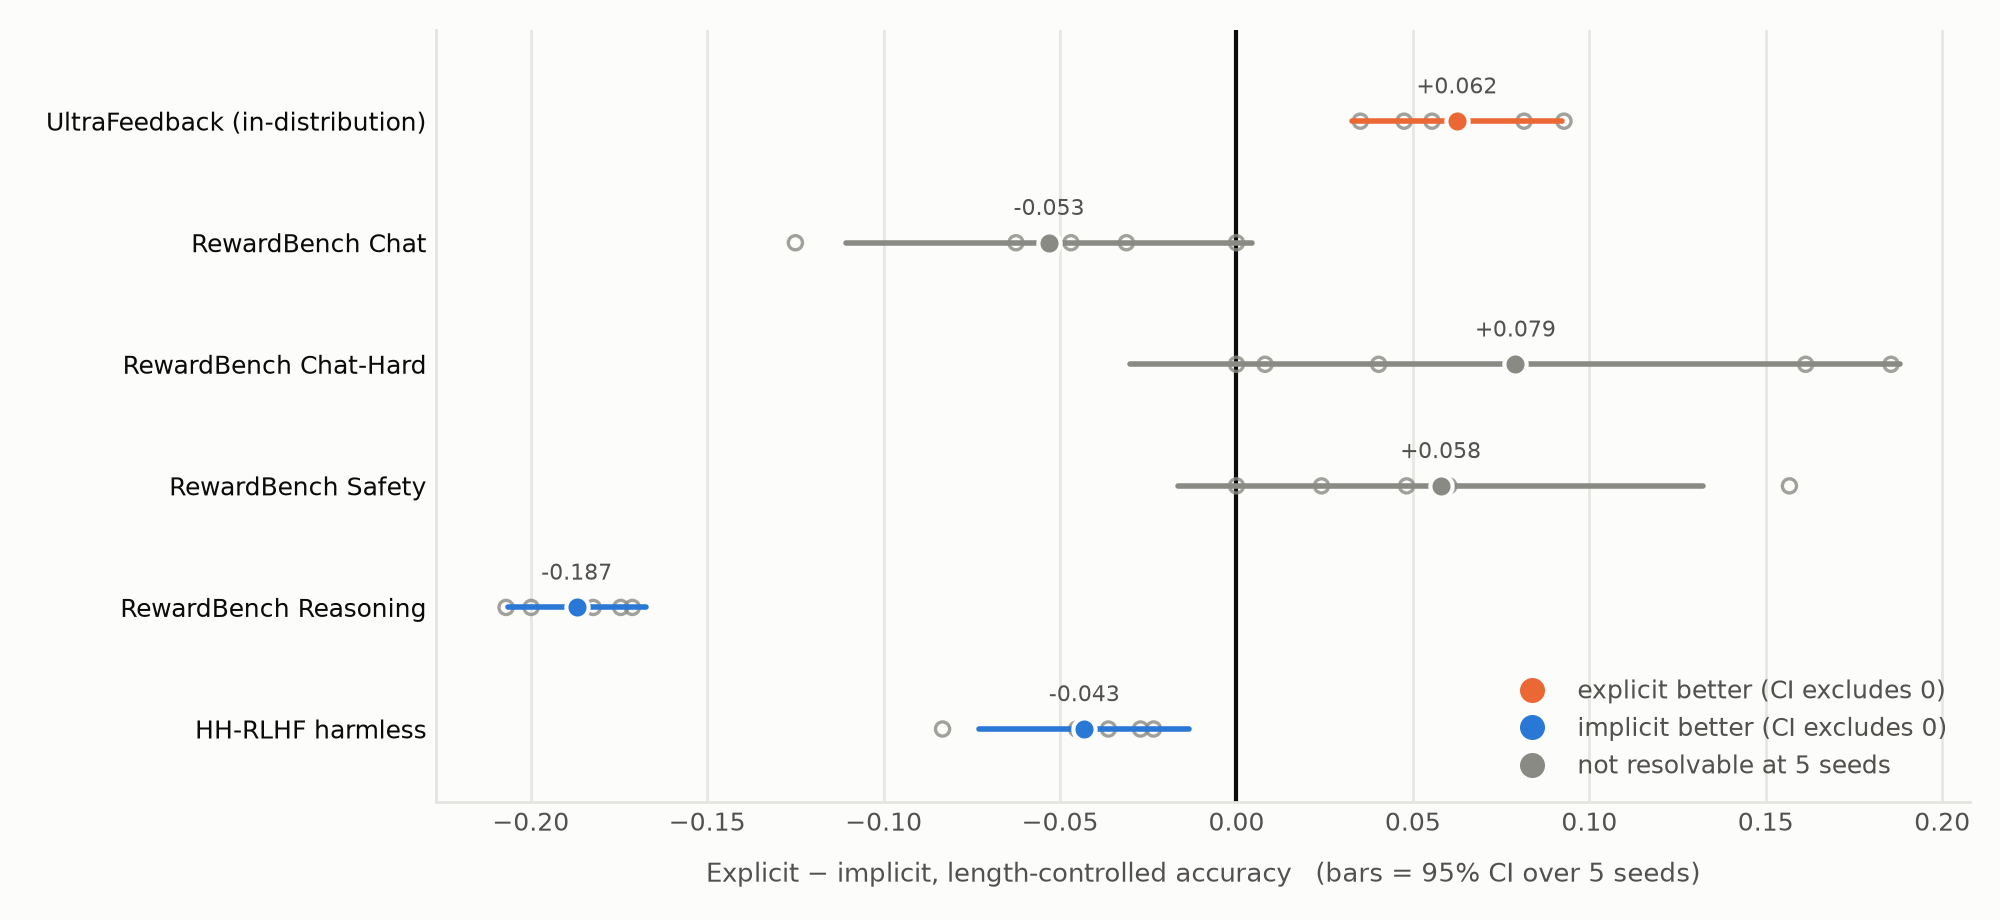
\includegraphics[width=0.82\linewidth]{figures/fig3_paired_delta.png}
\caption{Explicit minus implicit length-controlled accuracy, paired within each seed; bars
crossing zero (grey) are not resolvable.}
\label{fig:paired-delta}
\end{figure}

\subsection{An unplanned finding: reward training can underperform the SFT baseline}
Scored against the SFT log-probability baseline instead of chance, the baseline beats
\emph{both} trained scorers on RewardBench-Reasoning; on Chat-Hard it beats the implicit reward
resolvably, while the explicit model's gap is not resolvable (Figure~\ref{fig:value-added}).
Reward-model training, explicit or implicit, can therefore leave a scorer worse at ranking
preferences than the SFT policy's own untuned log-probability, on exactly the subsets
RewardBench designed to be hard and adversarial.

\begin{figure}[H]
\centering
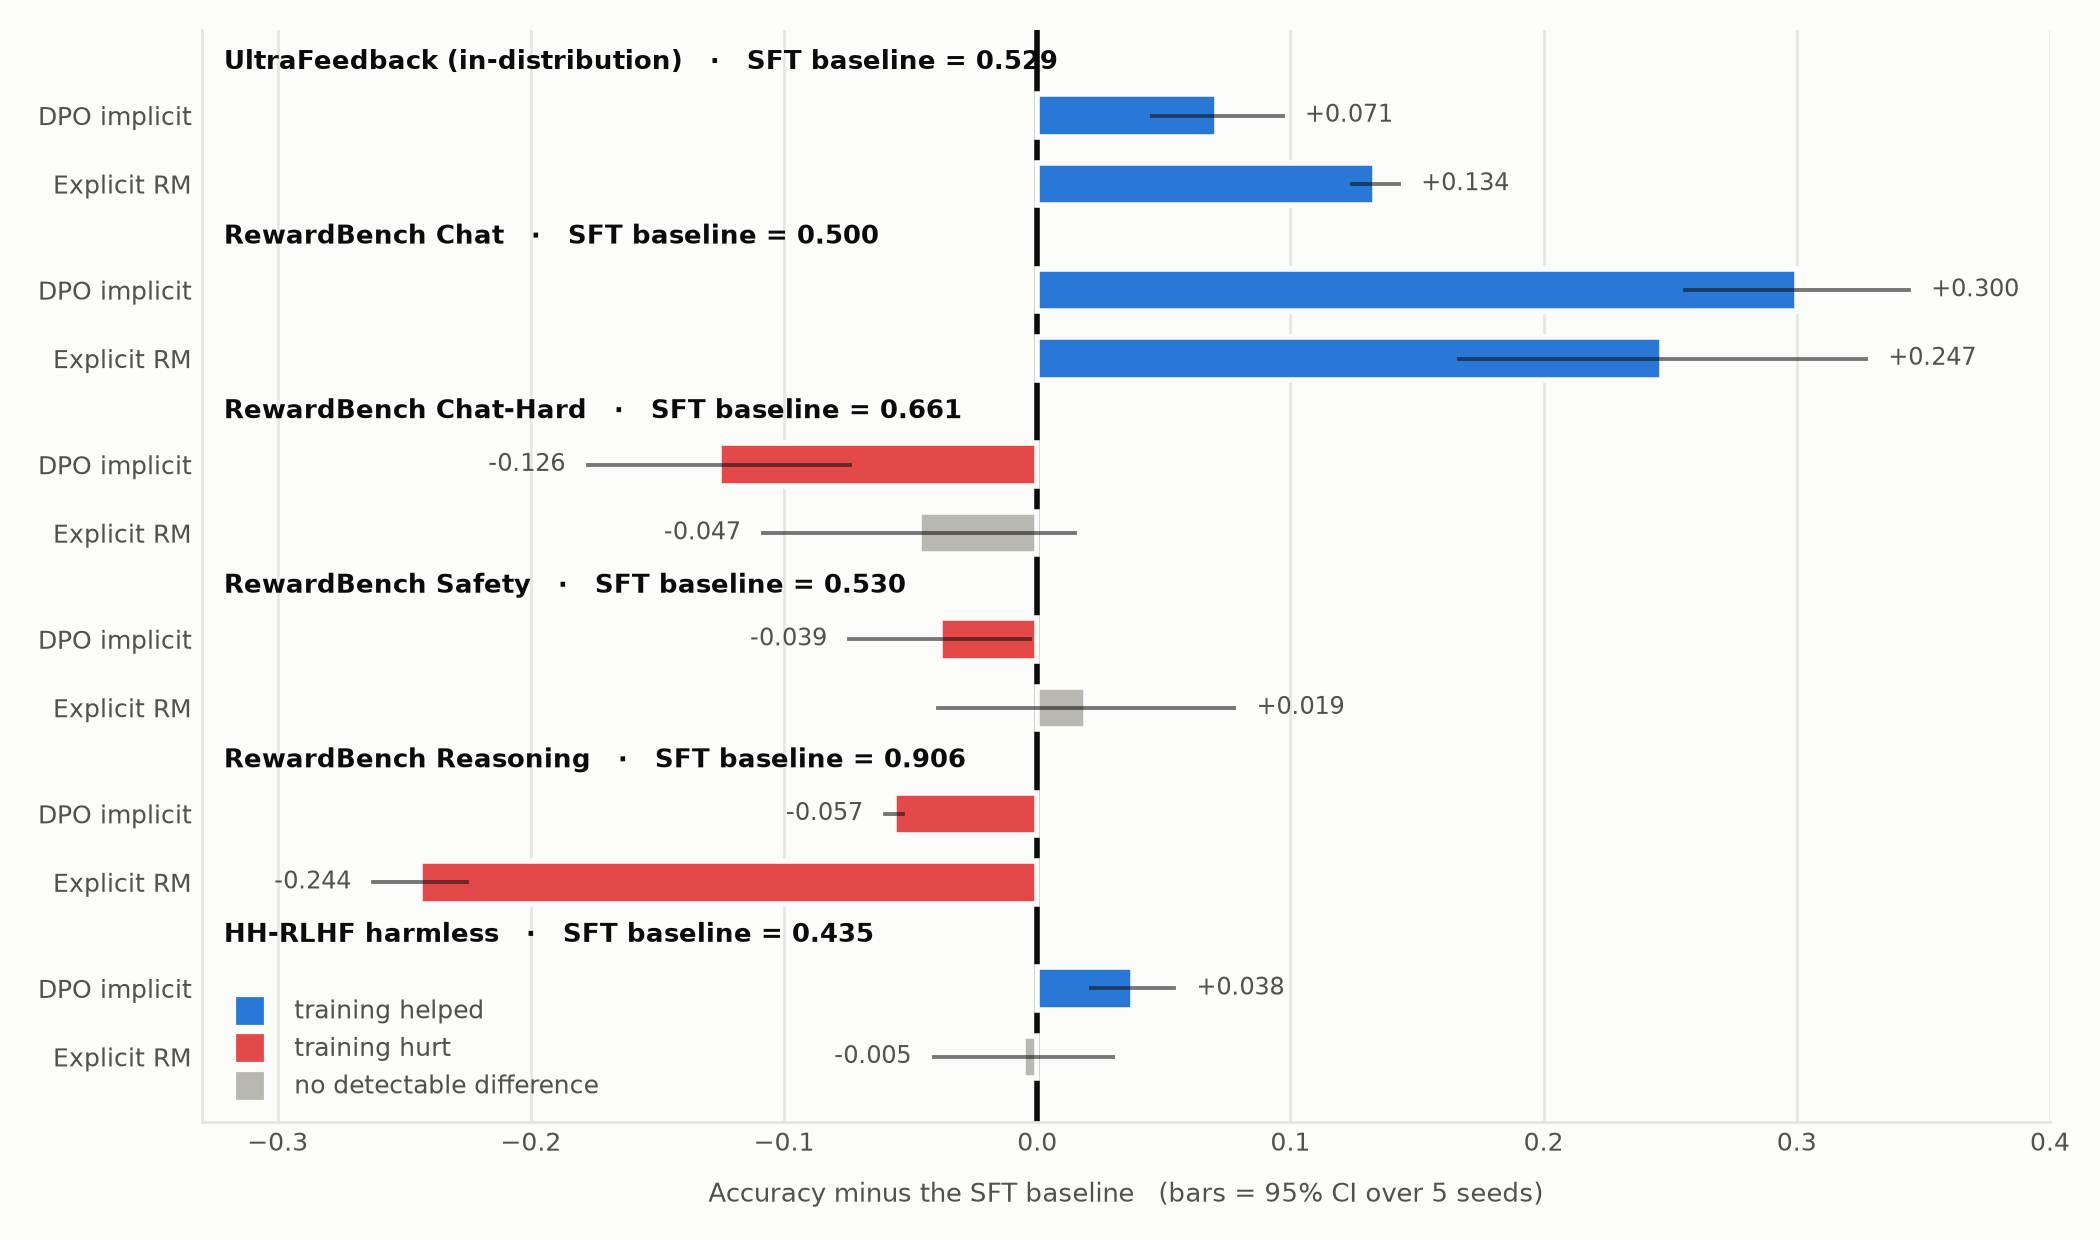
\includegraphics[width=0.82\linewidth]{figures/fig6_value_added.png}
\caption{Accuracy minus the SFT log-probability baseline; bars left of zero mean reward
training left the scorer \emph{worse} at ranking.}
\label{fig:value-added}
\end{figure}

\subsection{Length confound and surface-feature associations}
Length control matters: the explicit reward model scores below chance on Chat-Hard before
length control (0.414) and recovers once length-matched (Table~\ref{tab:results}), a shift
large enough to flip its ranking relative to chance. More generally, the explicit model and the
SFT baseline are both associated with preferring longer, more formatted, more numeric responses
relative to the human labels (10--16 points of deviation), while the implicit reward tracks the
human rate closely (Figure~\ref{fig:qualitative}). Response length is therefore one likely
contributor to H1's in-distribution gap and to the explicit model's raw-accuracy collapse on
length-inverted subsets like Chat-Hard.

\begin{figure}[H]
\centering
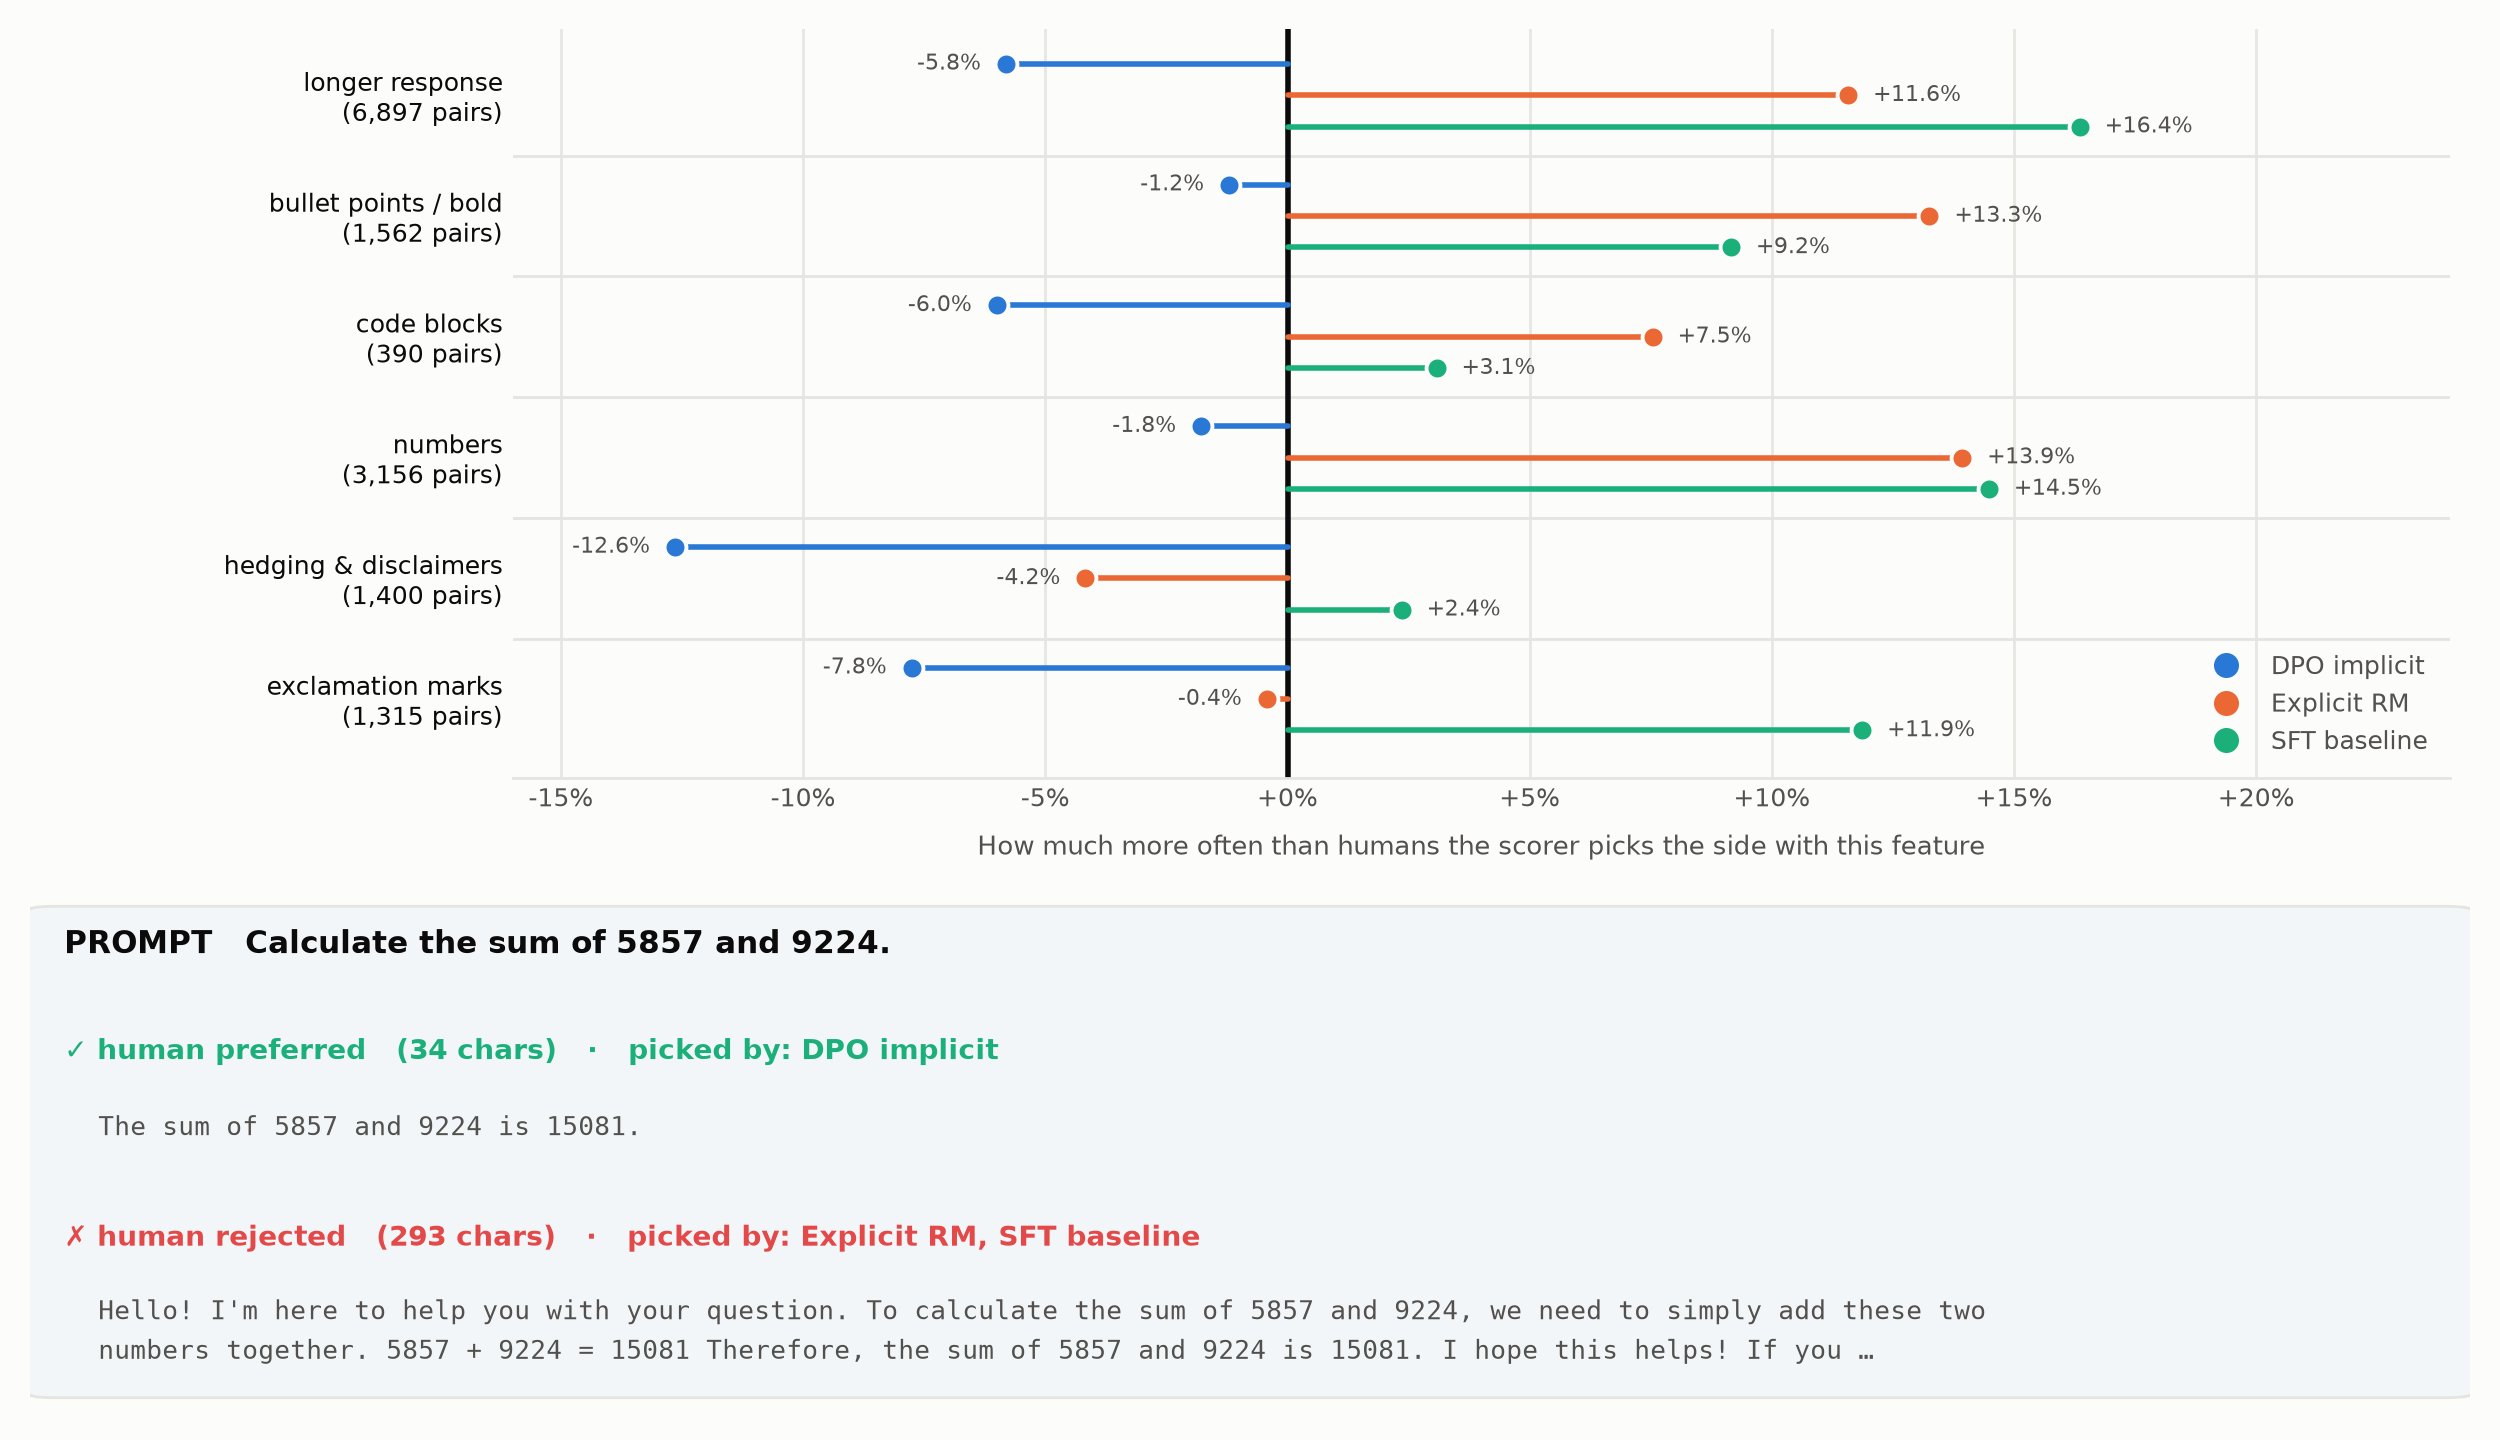
\includegraphics[width=0.96\linewidth]{figures/fig9_what_they_reward.png}
\caption{Deviation from the human rate on the same pairs, per surface feature (top), with one
worked example (bottom).}
\label{fig:qualitative}
\end{figure}

\subsection{Ablations: extended training and length-bias drift}
\label{sec:ablations}
Re-running both conditions for four epochs (two seeds), with held-out pairwise accuracy
measured every 100 steps on a shared 400-pair slice, tests whether the one-epoch ranking is an
artifact of stopping two still-improving models (Figure~\ref{fig:convergence}). The explicit
reward model climbs to a peak of $0.731$ near epoch 2 and then overfits; the implicit reward is
flat from the start, peaking at $0.676$ near epoch 1. The explicit model is ahead at every
epoch past $\sim$0.4: its lead is $\approx0.048$ at the one-epoch mark (0.724 vs.\ 0.676) and
$0.055$ at each method's own best checkpoint, slightly wider rather than
narrower.\footnote{Different metric and sample from Table~\ref{tab:results}'s $+0.062$; not
directly comparable.} \textbf{H1 remains supported through the full four-epoch run; the ranking
does not invert.} We stop short of calling this ``convergence'': the reward model is still
visibly overfitting, not plateaued, by epoch 4. Training loss keeps falling long after held-out
loss turns (Figure~\ref{fig:long-curves}), so it is not a usable stopping signal here; the
reward model's best checkpoint is near epoch 2, so four epochs is worse than one for it
specifically.

\begin{figure}[H]
\centering
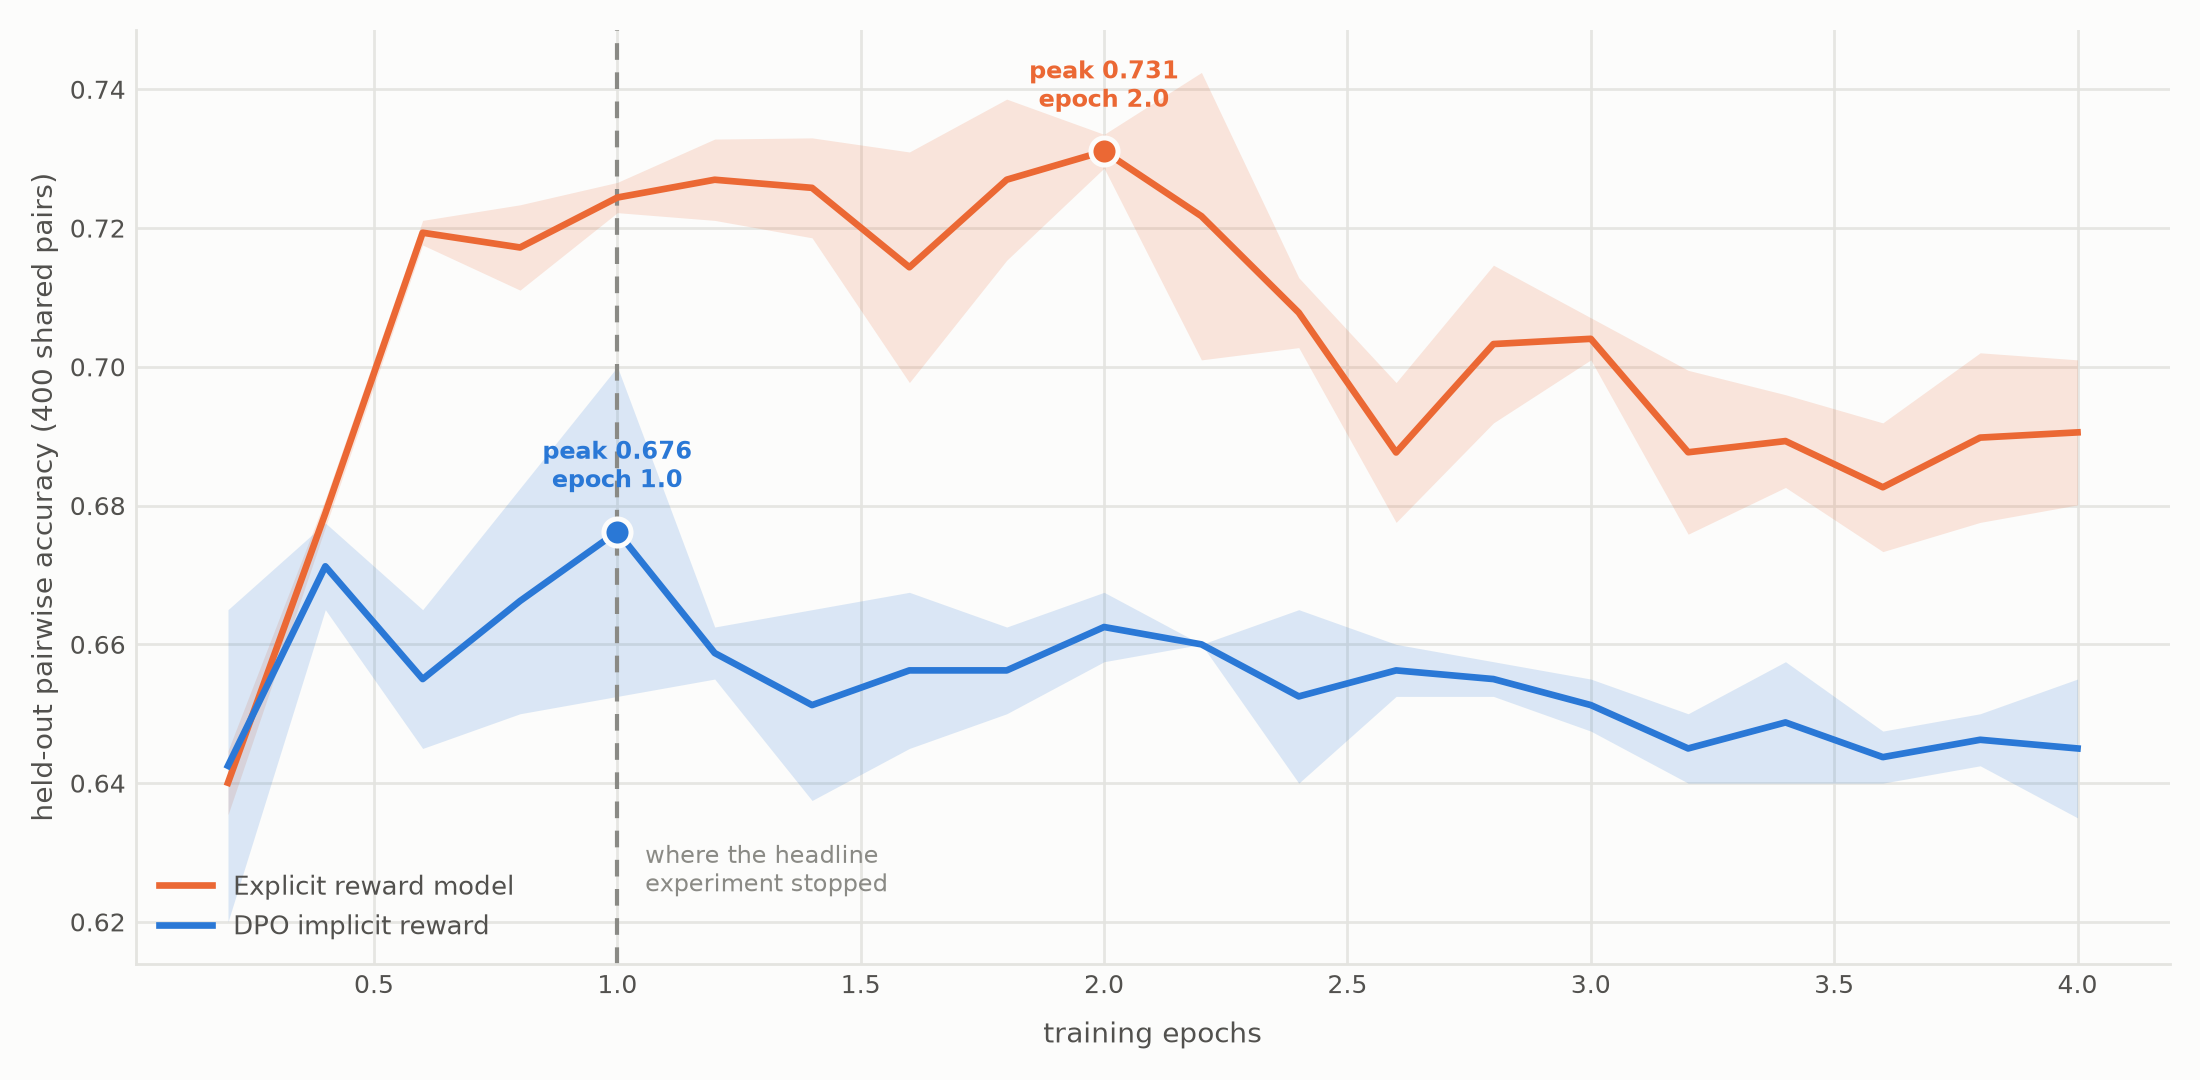
\includegraphics[width=0.78\linewidth]{figures/fig10_convergence.png}
\caption{Held-out pairwise accuracy across four training epochs; the band spans two seeds.}
\label{fig:convergence}
\end{figure}

\begin{figure}[H]
\centering
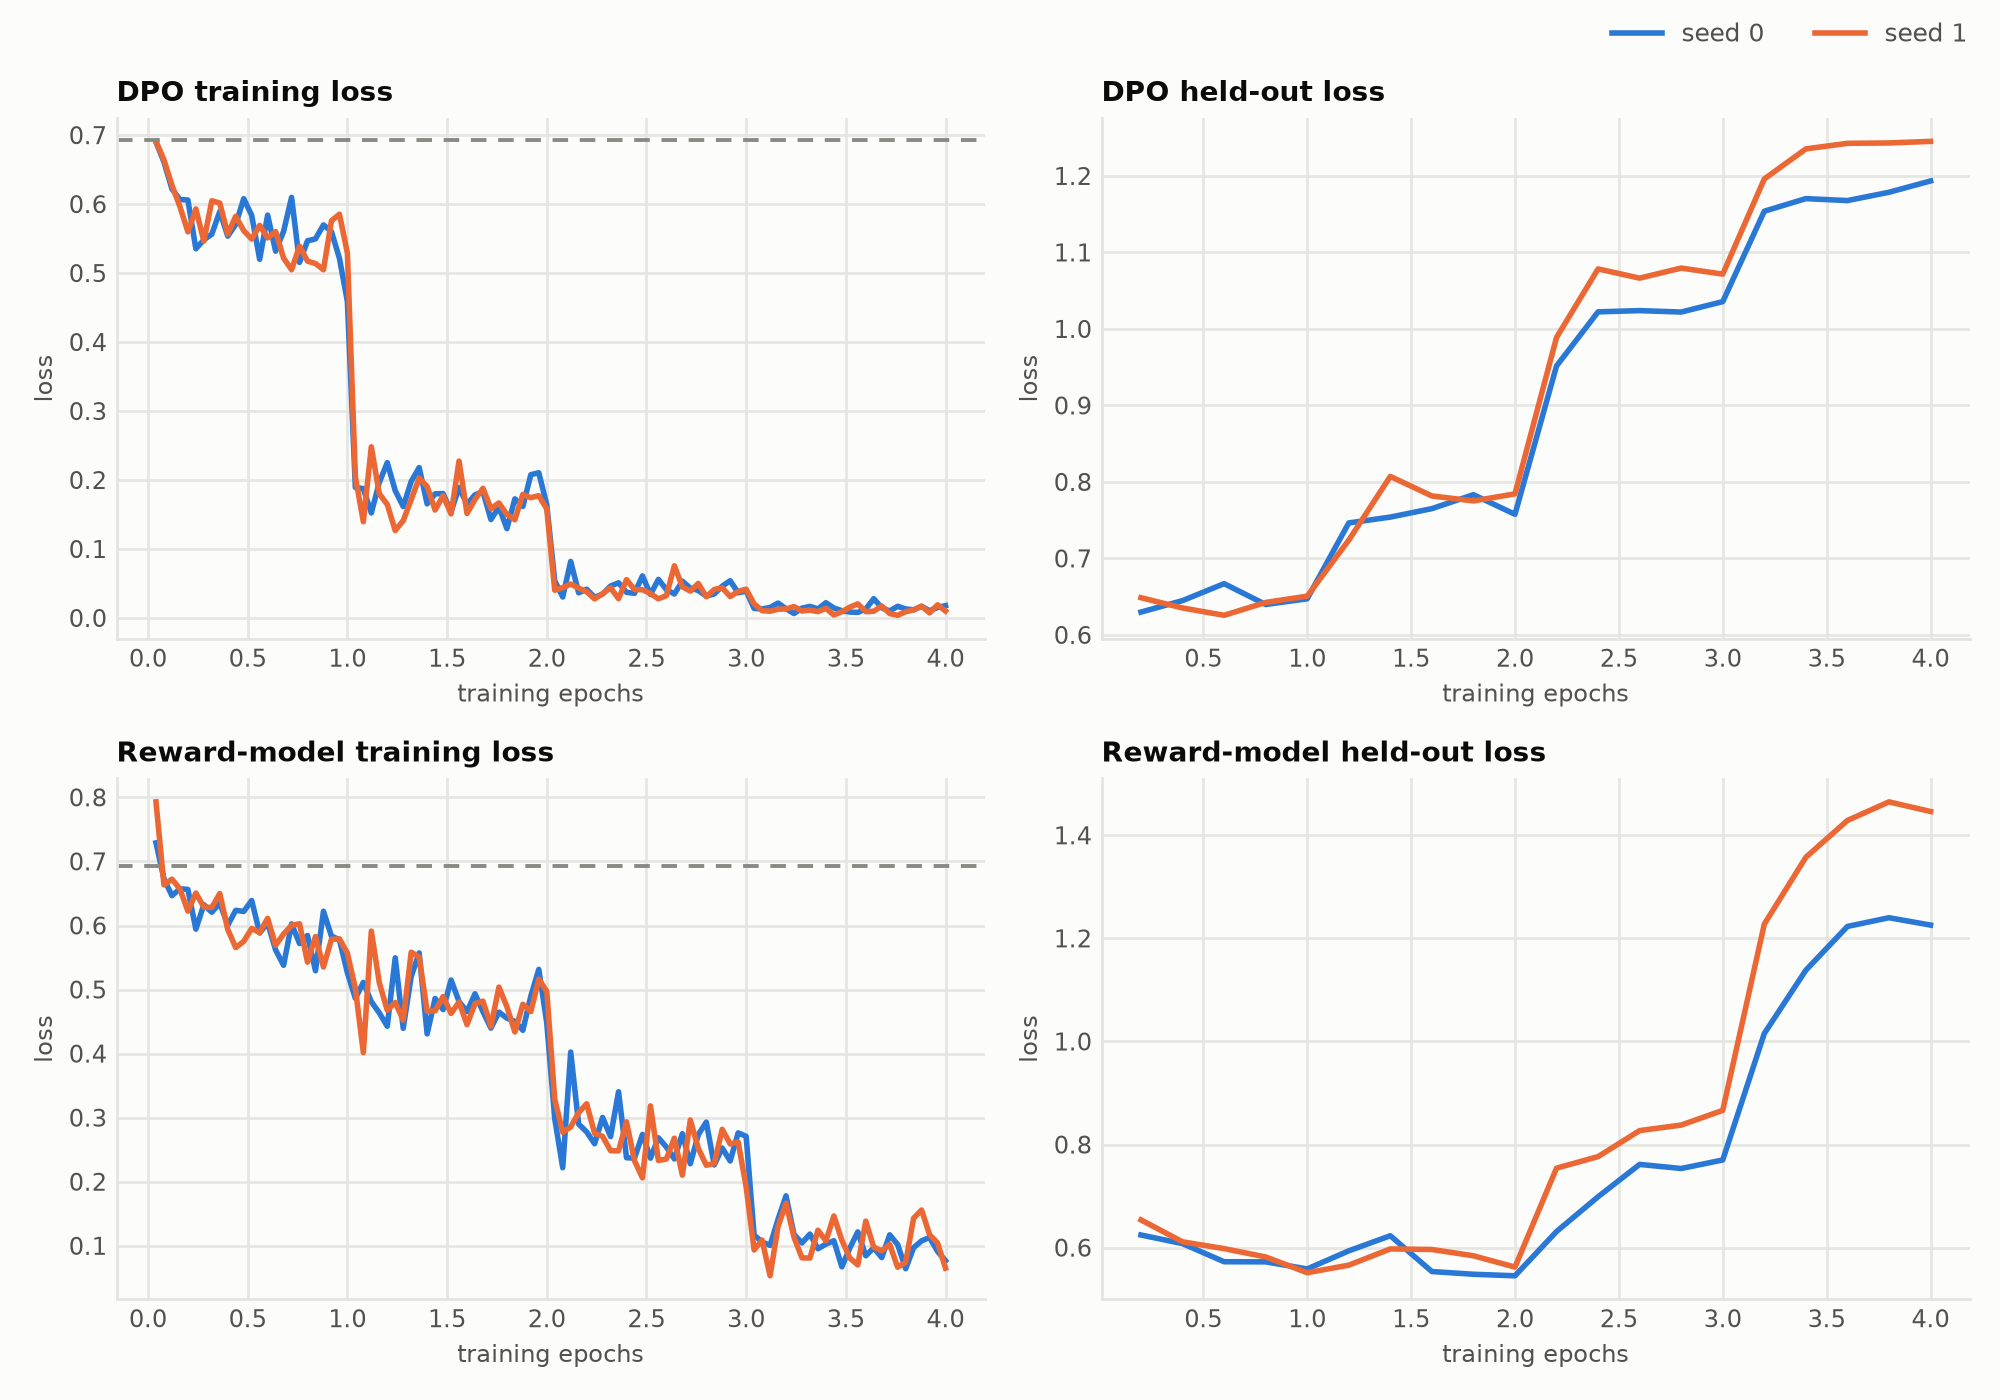
\includegraphics[width=0.80\linewidth]{figures/fig11_long_curves.png}
\caption{Training loss (left) against held-out loss (right) across the four-epoch run.}
\label{fig:long-curves}
\end{figure}

Scoring all eight saved checkpoints of each condition on 500 held-out pairs tests whether
either scorer's length bias grows with training (Figure~\ref{fig:bias-drift}; accuracy over the
same checkpoints: Figure~\ref{fig:convergence}). The hypothesis is \textbf{wrong for the
explicit model}: its length bias peaks early ($+0.069$ relative to the human rate at epoch 1.5)
and fades to $+0.002$ by epoch 4, on roughly the same schedule as its accuracy peaking and
falling. The implicit reward drifts the other way instead: its deviation from the human rate
moves from $-0.134$ to $-0.232$, so it ends up picking the \emph{longer} response only 32.5\%
of the time against a human rate of 55.7\%, with accuracy declining in step. This is consistent
with an anti-length preference induced by DPO training that contributes to why the implicit
reward saturates early and then degrades; both drifts are single-seed.

\begin{figure}[H]
\centering
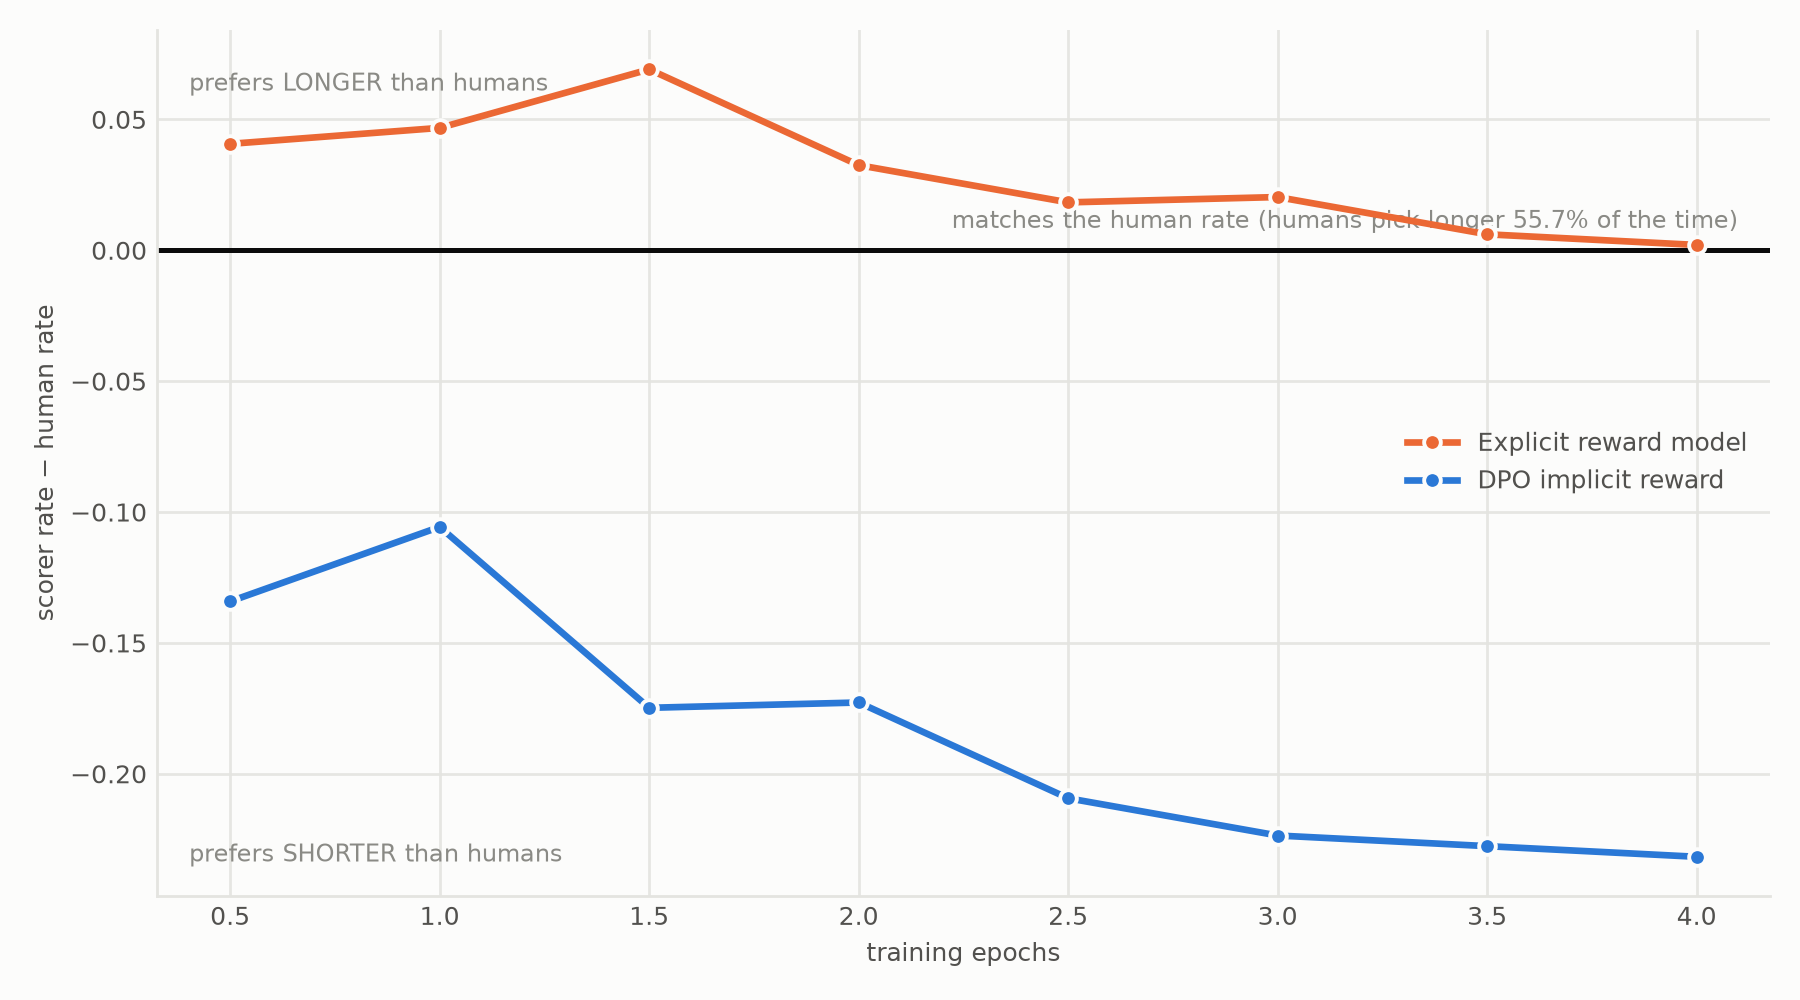
\includegraphics[width=0.72\linewidth]{figures/fig12_bias_drift.png}
\caption{Length preference relative to the human rate, across eight checkpoints per model.}
\label{fig:bias-drift}
\end{figure}

\subsection{Threats to validity}
\label{sec:threats}
Several limitations bound how far these results generalize.

\textbf{Sample size.} The three sets marked $^\dagger$ in Table~\ref{tab:datasets} fall below
100 length-matched pairs, the filter having removed up to roughly 90\% of each. Their
length-controlled numbers, reported to three decimals only for consistency with the rest of the
table, indicate direction rather than precise estimates; a length-adjusted regression, rather
than length filtering, would recover the lost statistical power.

\textbf{What is not matched.} Wall-clock time and total FLOPs are not matched, since DPO
performs an extra frozen-reference forward pass every step and took approximately $1.7\times$
the reward model's wall-clock time for the same optimizer steps. This is a matched
\emph{training budget} (Figure~\ref{fig:pipeline}), not matched compute in the FLOP sense.

\textbf{$\pi_{\mathrm{ref}}$ was trained once.} Seeds vary only the second-stage
(DPO/reward-model) training, so the reported intervals capture variance from that stage given
one fixed reference, not variance of the method as a whole --- which is also why the SFT
baseline's interval in Figure~\ref{fig:value-added} has zero width.

\textbf{Associations, not mechanisms.} The surface-feature effects in
Figure~\ref{fig:qualitative} are correlational and overlapping, since longer responses also
tend to contain more numbers and bullets, so isolating length would need a joint model.
Likewise the readings in \S3.5 and \S\ref{sec:ablations} of \emph{why} training degrades
performance, or why the implicit reward drifts toward shorter responses, are consistent with
the data rather than established causes.

\textbf{Calibration} is poor across the board (ECE 0.22--0.45 across scorers and sets), which
matters if the practical pitch is reusing either kind of scorer as a probability estimate
rather than only a ranker.

\textbf{Scope.} Every result is at one model scale (0.5B), one $\beta$ (0.1), and one training
budget (8{,}000 pairs); the $\beta \in \{0.05, 0.1, 0.3, 0.5\}$ and budget $\in \{2\text{k},
8\text{k}, 32\text{k}\}$ ablations planned in the proposal remain future work.

\section{Conclusion}
Budget-matched from one shared starting checkpoint (Figure~\ref{fig:pipeline}), an explicitly
trained Bradley--Terry reward model beats DPO's implicit reward on held-out, in-distribution
preference pairs, and the ranking survives an extended four-epoch run rather than reversing
(\textbf{H1 supported}). The predicted widening of that gap under distribution shift does not
occur; where a difference is resolvable, it favors the implicit reward instead (\textbf{H2 not
supported}). Unplanned, an SFT log-probability baseline with no reward-specific training beats
both trained scorers on the hardest, most adversarial subsets. DPO's ``secretly a reward
model'' claim therefore holds only in a narrow, in-distribution sense at this scale: an
explicit reward model is measurably better in distribution, but under shift neither trained
scorer consistently beats the untrained baseline, within the bounds of
\S\ref{sec:threats}. Future work should run the planned $\beta$/budget sweeps and re-seed the
reference policy itself so reported intervals describe the method rather than one
initialization.

\bibliography{myreferences}
\bibliographystyle{unsrt}
\end{document}
